%----------------------------------------------------------------------------------------
%	STEP BY STEP
%----------------------------------------------------------------------------------------

\textit{Ce projet est grandement inspiré d'un sujet proposé par \textit{Hervé SAUER} - enseignant-chercheur retraité de l'Institut d'Optique - en Calcul Scientifique il y a quelques années.}

\section{Introduction}

On se propose dans ce projet de simuler \textbf{l'éclairement} produit par un \textbf{ensemble de sources lumineuses incohérentes} sur un plan en deux dimensions.

\medskip

Ci-dessous une représentation de l'ambiance lumineuse basée sur la modélisation de sources lumineuses à l'aide d'un logiciel spécialisé de conception d'environnement d'éclairage en 3D - DIALux.

\begin{center}
	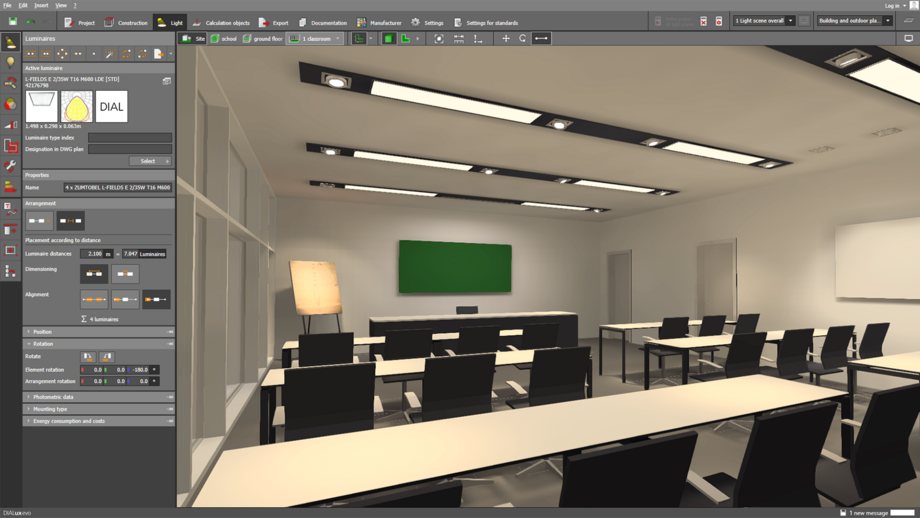
\includegraphics[width=7cm]{ \dirName /images/csm_DIALux-evo_Header_Scene-3-min_d6fe872b15.png}
\end{center}


\section{Objectifs}

\subsection{Modélisation simple}

Dans le cadre de ce projet, on souhaite obtenir une \textbf{cartographie en deux dimensions} (puis en trois dimensions selon l'ouverture choisie - voir paragraphe ouverture) d'un ensemble de sources à LEDs positionnées dans un espace en trois dimensions.

On partira d'un modèle simplifié d'une source lumineuse, repérée dans un espace en trois dimensions, dont la directivité de l'intensité sera perpendiculaire au plan de travail considéré et avec une intensité lumineuse donnée, pour ensuite enrichir le modèle en intégrant la possibilité de réorienter les sources par rapport à la normale du plan considéré.

Chaque source sera considérée comme indépendante des autres (incohérence) et il sera alors possible de complexifier le système en paramétrant un ensemble N de sources lumineuses et d'en obtenir la cartographie sur un plan donné.

\subsection{Conception de système d'éclairage}

Lorsque l'on conçoit un système d'éclairage, le but le plus souvent recherché est d'avoir un éclairement le plus uniforme et le plus lumineux possible sur une zone donnée en disposant de manière appropriée les sources dont on dispose. 

\medskip

A partir du modèle établi précédemment, il sera alors possible d'optimiser sous contrainte en minimisant la variance ou la valeur absolue de l'écart ou la valeur absolue de l'écart crête à la valeur moyenne de l'éclairement sur la zone considérée avec une contrainte d'éclairement moyen minimum et d'éventuelles contraintes supplémentaires sur le positionnement des sources pour modéliser des limitations ou impératifs mécaniques de placement de celles-ci.

\medskip

\textit{Par exemple, on pourra étudier le placement optimal sur un cercle de diamètre D et d'altitude z0 variables, de N DELs (par exemple, 5 ou 7) de même type (mêmes I0 et mêmes D), en fonction de la directivité des DEL (paramètre D), et de l'éclairement moyen (e.g. 10, 100 voire 1000 lux) souhaités sur un disque de diamètre d (3 ou 4 cm) donné... }


%%%%%%%%%%%%%%%%%%%%%%%
\section{Grandes étapes}

\begin{itemize}
	\item Définir une source lumineuse
	\item Définir un plan de travail
	\item Définir un système comprenant un plan de travail et un ensemble de sources lumineuses
	\item Calculer l'éclairement produit en tout point du plan de travail par chacune des sources lumineuses
	\item Calculer l'éclairement de l'ensemble des sources et afficher la carte
	\item Calculer la valeur moyenne et l'écart-type de l'éclairement produit
	\item Afficher les valeurs maximale, minimale ainsi que les moyennes et écart-type d'éclairement
\end{itemize}

\medskip

\textit{Afin de simplifier la phase de développement et d'essais de votre application, nous vous suggérons de commencer à réaliser vos modélisations de la façon suivante : }

\begin{description}
	\item[Essai 1] Carte d'éclairement pour une source ponctuelle - direction perpendiculaire par rapport au plan éclairé
	\item[Essai 2] Carte d'éclairement pour une source ponctuelle - direction quelconque par rapport au plan éclairé
	\item[Essai 3] Carte d'éclairement pour N sources ponctuelles - direction quelconque par rapport au plan éclairé
\end{description}

%%%%%%%%%%%%%%%%%%%%%%%
\section{Modélisation des sources et calcul d'éclairement}

\subsection{Modélisation d'une diode électroluminescente}


Les sources seront modélisées de manière approchée (valable si l'on n'est pas trop près du composant) comme une \textbf{source ponctuelle} ayant un diagramme de rayonnement possédant une symétrie de révolution autour d'un axe.

Les sources (par exemple des LEDs) seront modélisées de manière approchée (valable si l'on n'est pas trop près du composant) comme des \textbf{sources ponctuelles}. Ces sources ont un \textbf{diagramme de rayonnement} possédant une \textbf{symétrie de révolution} autour d'un axe orienté. 

\medskip

L'indicatrice de rayonnement pourra être considérée comme gaussienne, et caractérisée par son intensité visuelle vers l'avant sur l'axe $I_0$ (en candela) et sa largeur totale à mi-hauteur $\Delta$.

Cette indicatrice peut-être modélisée par l'équation suivante : $$I(\alpha) = I_0 \cdot \exp(-(4 \cdot \ln(2)) \cdot (\alpha/\Delta)^2)$$

où $\alpha$ est l'angle entre la direction d'émission et l'axe de la source ($\alpha \in [0^{\circ}, 180^{\circ}]$). 

\medskip

%%%%%%%%%%%%%%%%%%%%%%%
\subsection{Positionnement d'une source}

Le positionnement de la source dans l'espace sera caractérisé par ses coordonnées $(x, y, z)$ et l'orientation de son axe de symétrie par deux angles ($\theta$ et $\phi$). 
	
\medskip

%%%%%%%%%%%%%%%%%%%%%%%
\subsection{Eclairement / Formule de Bouguer}

L'éclairement fourni par une source ponctuelle en un point M de l'espace séparé d'une distance $d$ et d'une inclinaison de $\psi$ par rapport à la direction de la source ponctuelle, est données par la relation photométrique suivante : 

$$E = \frac{I \cdot \cos(\psi)}{d^2}$$


%%%%%%%%%%%%%%%%%%%%%%%

L'éclairement produit par N sources (incohérentes) est la somme des éclairements produits par chaque source.

\medskip


%%%%%%%%%%%%%%%%%%%%%%%
\textit{Les représentations graphiques à produire à chacune des étapes seront accompagnées de \textbf{renseignements quantitatifs} comme la valeur moyenne de l'éclairement, son écart-type et son écart Pic à Vallée, absolus et relatifs, sur l'ensemble de la zone représentée (ou sur une sous-partie rectangulaire ou circulaire de celle-ci). Par ailleurs, une \textbf{représentation en 3D de la position et de l'orientation des N sources} sera utile.}


%%%%%%%%%%%%%%%%%%%%%%%
\section{Quelques pistes d'ouvertures possibles}

\textbf{Vous devrez choisir et réaliser au moins l'une des ouvertures suivantes dans le cadre de ce projet}.

\begin{description}

	\item[Ouverture A] \textbf{Carte d'éclairement 3D}
	
	\begin{itemize}
		\item Affichage 3D d'une carte avec une source ponctuelle avec position des sources sur la carte
	\end{itemize}	

\qquad

	\item[Ouverture B] \textbf{Optimisation d'un éclairement}
	
	\begin{itemize}
		\item Optimisation du nombre et de l'orientation de LEDs pour obtenir un flux lumineux donné sur un plan de travail
	\end{itemize}	

\qquad
	
	\item[Ouverture C] \textbf{Plusieurs plans de travail}
	\begin{itemize}
		\item Système final avec plusieurs plans de travail à des hauteurs différentes par exemple
		\item Prise en compte de l'ombre portée d'un plan sur un autre
	\end{itemize}
	
\end{description}


%%%%%%%%%%%%%%%%%%%%%%%%%
\section{Critères d'évaluation}

\textbf{Grille à simplifier (bilan Semestre 5)}

\begin{itemize}
	\item \textbf{METHODES NUMERIQUE}
	\begin{itemize}
		\item \textbf{Ecriture Matricielle / Vectorielle}
		\begin{itemize}
			\item utilisation des méthodes liées aux vecteurs/matrices (Numpy)
			\item aucune boucle \textbf{for} inutile
		\end{itemize}		 
		\item \textbf{Organisation en actions élémentaires}
		\begin{itemize}
			\item les étapes sont découpées en fonctionnalité plus simple à tester
		\end{itemize}
		\item \textbf{Description des tests de validation}
		\begin{itemize}
			\item chaque fonction a été testée
			\item chaque étape a été validée
		\end{itemize}
		\item \textbf{Organisation des informations à traiter}
		\begin{itemize}
			\item les données sont rangées dans des objets bien identifiés
		\end{itemize}
	\end{itemize}


	\item \textbf{PROGRAMMATION}
	\begin{itemize}
		\item \textbf{Ecriture globale du code et commentaires (PEP 8)}
		\begin{itemize}
			\item variables et fonctions respectant les conventions d'écriture standard
			\item commentaires utiles
		\end{itemize}		 
		\item \textbf{Utilisation, écriture de fonctions}
		\begin{itemize}
			\item paramètres et retours pertinents des fonctions
		\end{itemize}
		\item \textbf{Documentation des fonctions (PEP257)}
		\begin{itemize}
			\item paramètres et retours des fonctions sont documentés
		\end{itemize}
		\item Création de classes et d'objets
		\begin{itemize}
			\item classe contenant des attributs et méthodes pertinents
			\item aucune fonction n'est appelée en dehors d'un objet
		\end{itemize}
	\end{itemize}
	

	\item \textbf{INGENIEUR.E PHYSIQUE}
	\begin{itemize}
		\item \textbf{Graphiques pertinents et légendés}
		\begin{itemize}
			\item graphiques scientifiques (axes, titre...)
			\item axes des graphiques légendés (passage temps/fréquence)
		\end{itemize}		 
		\item \textbf{Organisation en actions élémentaires}
		\begin{itemize}
			\item les étapes sont découpées en fonctionnalité plus simple à tester
		\end{itemize}
		\item \textbf{Génération de données pertinentes de tests}
		\begin{itemize}
			\item choix de la position des sources pertinent
		\end{itemize}
		\item \textbf{Analyse des données et validation modèle}
		\begin{itemize}
			\item comparaison avec la théorie
			\item analyse pertinente des cartes obtenues
		\end{itemize}
	\end{itemize}
	
\medskip	
	
	\item \textbf{AVANCEMENT}
	\begin{itemize}
		\item Etapes 1 et 2 : x 0.5
		\item Etapes 1, 2 et 3 : x 0.7
		\item Une des ouvertures : x 1.0
	\end{itemize}
\end{itemize}



